\pagestyle{plain}
\setcounter{page}{1}
\pagenumbering{arabic}
% \thispagestyle{empty}\section{Introdução}
	A utilização da liga FeSi com 75\% de silício foi introduzida em abril de 2012 para reduzir o consumo de alumínio nos aços acalmados ao alumínio (AA) produzidos no desgaseificador RH. Esta técnica permitiu reduzir o consumo de alumínio de 3,1 kg/t para 2,4 kg/t\cite{follow12}. A justificativa econômica reside na diferença de custo entre as ligas. Apesar de possuir um custo menor, a desoxidação com FeSi gera menos calor, o que pode ser um complicador pois não é vantajoso utilizar o FeSi quando levar a um aquecimento posterior do aço. Se for preciso aquecer o aço com oxigênio após a desoxidação haverá perda de limpidez pela geração tardia de inclusões de alumina. Se, por outro lado, nenhum aquecimento for necessário então haverá um ganho de qualidade pois a geração total de alumina será menor.
	
	No final de 2103, foi detectado que o consumo de alumínio nos aços UBC (Ultra Baixo Carbono) havia retornado ao patamar anterior ao projeto de redução de consumo de alumínio\cite{repnov}. Uma investigação \cite{prop} mostrou que a proporção de corridas caiu de 47\% em janeiro para 25\% em novembro de 2013. 
	
	Para otimizar a utilização do FeSi propõe-se um critério objetivo baseado dos resultados das corridas de 2013. Um modelo matemático para a tomada de decisão sobre quando utilizar o FeSi foi desenvolvido utilizando a técnica de regressão logística binária. 
\section{Métodos}		
	Para auxiliar a tomada de decisão quanto a utilização do FeSi foi implementado um algorítmo de classificação baseado na técnica de regressão logistica binária\cite{wiki:lr}. O fundamento da regressão logística binária é encontrar o conjunto de coeficientes para uma equação linear que melhor ajusta o logarítmo das chances em favor de um evento. No problema da utilização da liga de FeSi o evento é a utilização da liga. A definição de chance dada de acordo com a Equação (\ref{eq:odds}):	
	\begin{equation}
		\label{eq:odds}
		c = \frac{p}{1-p},
	\end{equation}
	\noindent onde $c$ é a chance e $p$ é a probabilidade a favor do evento. De acordo com a Equação (\ref{eq:odds}), para um evento muito provável quando $p \rightarrow 1$ então $c \rightarrow \infty$; e para um evento improvável $ c \rightarrow 0$. 
	
	A forma elementar para o modelo de regressão logística é dada pela Equação (\ref{eq:model}):	
	\begin{equation}
		\label{eq:model}
		\ln \left( \frac{p}{1-p} \right) = a_0 + a_1 x_1 + a_2 x_2 + ... + a_n x_n,
	\end{equation}	
	\noindent onde $a_0, a_1, ..., a_n$ são os parâmetros a serem ajustados e $x_1, x_2, ..., x_n$ são os valores das $n$ variáveis explicativas escolhidas para realização da regressão. 
	
	As variáveis escolhidas para realização da regressão logística foram: (1) Temperatura do último Celox antes da desoxidação, em ºC; 
	(2) Concentração de oxigênio livre do último celox antes da desoxidação, em ppm; (3) Temperatura de liberação (última medição da corrida), em ºC.
	% trim sequence: left, bottom, right and top
	\begin{figure}[H]
		\centering
		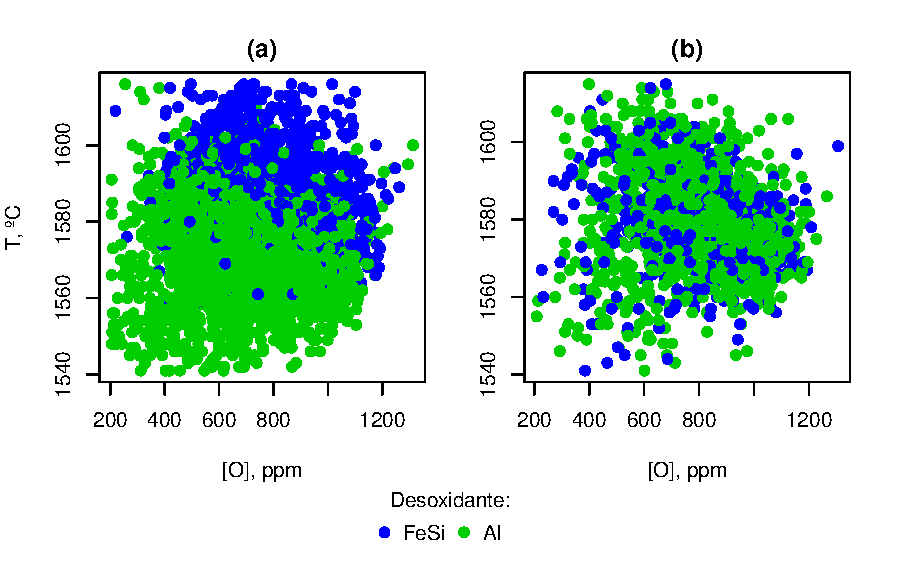
\includegraphics[scale=0.55, bb=0 0 432 280, trim=0in 20pt 0in 0in]{figures/fig01.pdf}
		\caption{Medição Celox anterior à desoxidação: (a) corridas ideais e  (b) corridas com correção.}
		\label{fig:ace}
	\end{figure}		
	Foram coletadas 5386 corridas AA-UBC que foram, então, classificadas em duas categorias: (a) corridas ideais onde a decisão foi acertada e (b) corridas em que a decisão não foi acertada. A Tabela (\ref{tab:um}) apresenta um resumo dos critérios que utilizados para classificar as corridas e o número de observações em cada caso. Nas corridas em que não houve aquecimento ou resfriamento, a decisão foi considerada acertada independente desta ter sido em favor do FeSi ou não. Nas corridas em que, após a desoxidação houve aquecimento e resfriamento foi considerado erro. Também configura acerto as corridas sem FeSi e com aquecimento e as com FeSi seguido de resfriamento.

	Na Figura (\ref{fig:ace}) são apresentadas as últimas medições Celox antes da desoxidação com seus valores de temperatura e concentração de oxigênio livre nos eixos vertical e horizontal, respectivamente separado em dois casos: no painel (a) as corridas em que a decisão foi tomada corretamente segundo os critérios apresentados na Tabela (\ref{tab:um}) e em (b) as corridas em que a decisão não foi tomada corretamente. 	
	\begin{table}[H]		
		\caption{Critérios para classificação das corridas entre corridas ideais (a) e corridas indesejáveis (b) e o número de corridas em cada caso.}
		\label{tab:um} % the label needs to be after the caption
		\begin{tabular}{lcccc}
		\hline 
		Desoxidante 					& Sopro                & Canivete             & Ambos                & Nenhum               \\
		\hline \hline 
		Al                              & (a) 1920             & (b) 479              & (b) 217              & (a) 811              \\
		FeSi                            & (b) 735              & (a) 585              & (b) 123              & (a) 516              \\
		\hline 
		\end{tabular}
	\end{table}	
	Para o treinamento do modelo de tomada de decisão, foram utilizadas as 3832 corridas em que a decisão foi acertada.	Os valores ótimos para os parâmetros do modelo foram obtidos utilizando o pacote estatístico de código livre \textit{RStudio} juntamente com a linguagem de programação R\cite{rprog}. Foi utilizada a função \texttt{glm()} para encontrar o conjunto de coeficientes que minimiza o erro quadrático médio.
	\begin{figure}[H]
		\centering
		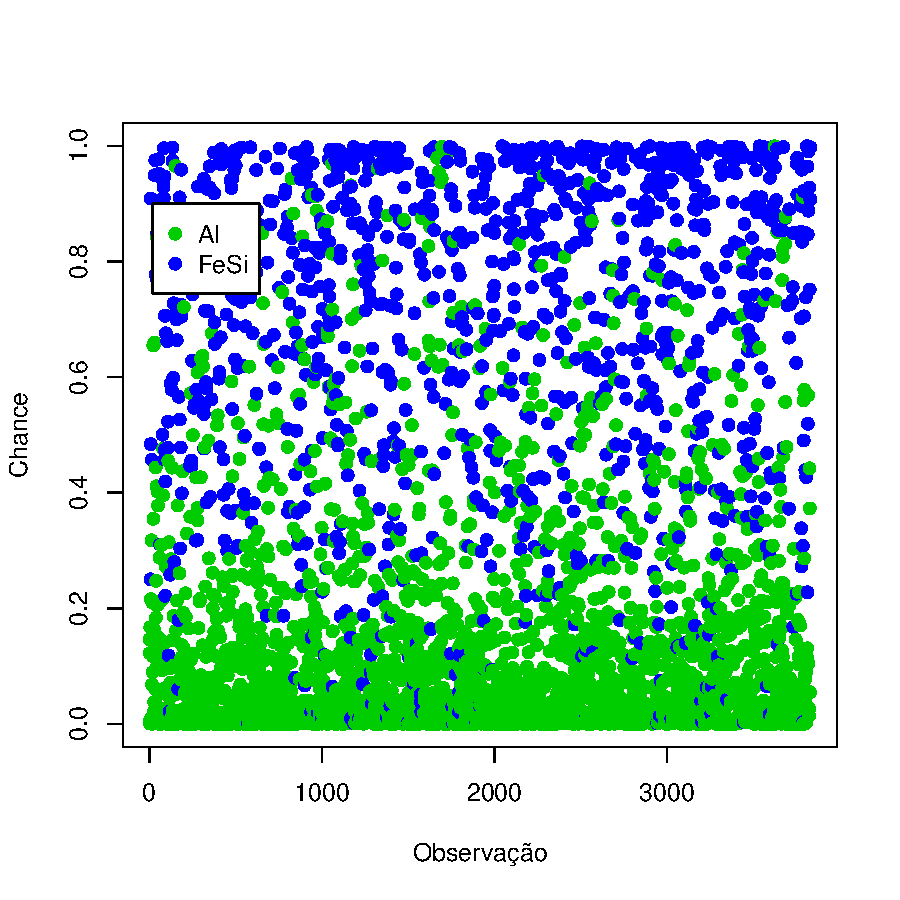
\includegraphics[scale=0.55, bb=0 0 432 432, trim=0in 20pt 0in 40pt]{figures/fig02.pdf}
		\caption{Probabilidade, $p$ calculado com base na chances prevista pela regressão logística binária e resultado real da utilização do FeSi (cores).}
		\label{fig:razao}
	\end{figure}		
\section{Resultados}
	O resultado da aplicação da função \texttt{glm()} aos dados de treinamento é sumarizado na Tabela (\ref{tab:result}). Os valores de Z apresentados juntamente com os valores dos parâmetros dão uma indicação de quão extremos são os valores dos parâmetros em relação ao acaso.
	\begin{table}[H]
		\centering
		\caption{Coeficientes do modelo de regressão logística binária juntamente com o valor de Z.}
		\label{tab:result}
		\begin{tabular}{lcc}
			\hline
			Coeficiente 			& Valor 					& Z  	\\
			\hline \hline
			\textit{(intercepto)}	& $-1.497$					& $-1.019$	\\			
			Temperatura 			& $ 2.072 \times 10^{-1}$	& $28.199$	\\
			Oxidação    			& $ 8.345 \times 10^{-3}$	& $21.499$	\\
			Temp. Liberação			& $-2.013 \times 10^{-1}$	& $-18.401$	\\			
			\hline \hline
		\end{tabular}
	\end{table}	
	Os valores listados na Tabela (\ref{tab:result}) foram utilizados com os dados de treinamento para calcular a chance de acerto na tomada de decisão. A chance calculada desta maneira foi utilizada para se obter o valor da probabilidade de utilização correta de FeSi utilizando a Equação (\ref{eq:odds}). A probabilidade de utilização correta juntamente com a decisão real é mostrada na Figura (\ref{fig:razao}).
	Fica evidente na Figura (\ref{fig:razao}) que a aplicação do modelo de regressão logística consegue de fato separar as corridas com e sem a utilização de FeSi. Quando o valor calculado para a chance $c$ é próximo de zero a melhor decisão é utilizar somente alumínio e quando o valor de $c$ é próximo de um a melhor decisão é pela utilização da liga FeSi. Para valores intermediários de $p$ há um confundimento aparente. Portanto, para permitir a utilização do modelo na prática é preciso determinar um valor limiar de $p$ para separar as duas regiões. A escolha do valor limiar de $p$, $p_l$ requer que seja definido um critérnio objetivo de precisão para o modelo de classificação.
	\begin{figure}[H]
		\centering
		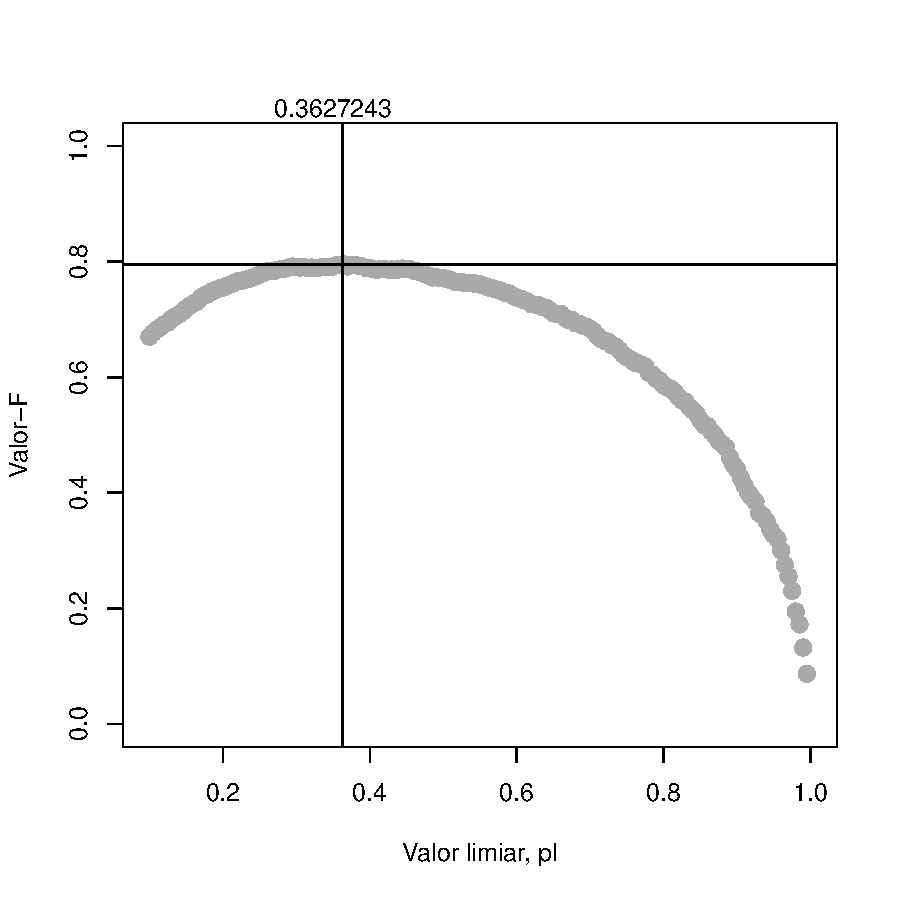
\includegraphics[scale=0.55, bb=0 0 432 432, trim=0in 20pt 0in 40pt]{figures/fig03.pdf}
		\caption{Valor do escore $F$ para diferentes valores de $p_l$. O valor ótimo para $p_l$ é aquele que maximiza o escore $F$.}
		\label{fig:sa}
	\end{figure}	
	Um critério comumente usado para avaliar a qualidade de um modelo de classificação binário é o da precisão/exaustividade\cite{wiki:pr}. Este critério implica na escolha do valor $p_l$ tal que a função $F$ é maximizada, onde:
	\begin{equation}
		\label{eq:defF}
		F=2\times\frac{pr}{p+r},
	\end{equation}
	\noindent onde $p$ é a precião do modelo e $r$ é a exaustividade. Mais detalhes sobre o escore $F$ podem ser encontrados em outra parte\cite{wiki:pr}.
	
	A determinação do valor ótimo de $p_l$ foi realizado de modo iterativo no ambiente \textit{RStudio}. Foram calculados os escores $F$ para valores de $p_l$ entre 0,1 e 1,0 com passo de 0,01 juntamente com a função \texttt{optimize()}. A Figura (\ref{fig:sa}) mostra a relação entre o escore $F$ e o valor limiar de $p$. O valor obtido para $p_l$ foi de 0,3627243.

	A proporção atual de acertos na decisão de utilizar ou não o FeSi foi calculada com base na Tabela (\ref{tab:um}) onde o total de corridas classificadas como (a) foi dividido pelo número total de corridas. O percentual atual de acertos foi de 71,1\% dos casos. A aplicação do modelo de classificação binário nos dados de treinamento resultou em um acerto de 87,5\%.
	
	A Equação (\ref{eq:reesc}) é usada para representar as regiões de decisão para temperaturas de liberação fixas. Esta relação foi obtida manipulando-se a Equação (\ref{eq:model}).
	\begin{equation}
		\label{eq:reesc}
		T = \frac{1}{a_1} \left[ \ln \left( \frac{p_l}{1-p_l} \right) - a_0 - a_2 O - a_3 T_l \right],
	\end{equation}
	\noindent onde $T$ é a temperatura do Celox antes de desoxidar em ºC, $T_l$ é a temperatura de liberação em ºC e $O$ é a concentração de oxigênio libre em ppm. A Figura (\ref{fig:level}) é a representação da Equação (\ref{eq:reesc}) para algumas temperaturas. O FeSi deverá ser utilizado sempre que a medição Celox anterior à desoxidação estiver acima da curva de nível correspondente à temperatura de liberação desejada.
	\begin{figure}[H]
		\centering
		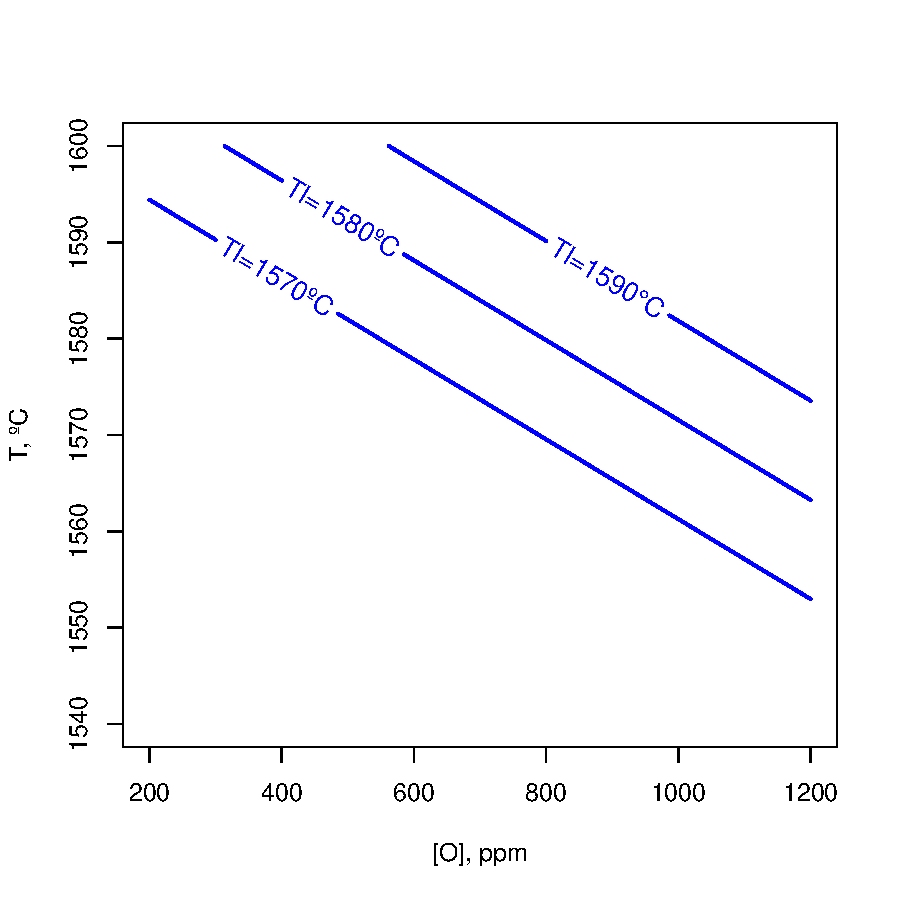
\includegraphics[scale=0.55, bb=0 0 432 432, trim=0in 20pt 0in 40pt]{figures/fig05.pdf}
		\caption{Curvas de iso temperatura de liberação: usar FeSi sempre que o Celox medido antes da desoxidação estiver acima da respectiva curva de nível.}
		\label{fig:level}
	\end{figure}	
\section{Conclusão}
	Foi desenvolvido um modelo de classificação baseado na técnica de regressão logística binária para decidir com base na última medição Celor antes da desoxidação e na temperatura de liberação desejada quando utilizar a liga FeSi para pré-desoxidação de aços AA no desgaseificador RH.
	
	O valor limiar para a razão de chance foi escolhido pela maximização da função $F$ que representa a média harmônica entre a precisão e exaustividade\cite{wiki:pr}. A taxa de acerto do modelo foi estimada em 87,5\% com os dados de treinamento o que representa um potencial de melhoria diante do patamar atual de 71,1\%.